\section{Experiments}
\label{sec:experiments}

We organize the experiments to mirror this narrative: we first report a controlled support-context study that establishes the motivating phenomenon, then the main comparison against state-of-the-art methods across six domains, followed by the prototype-space and hyper-parameter analyses, and finally a component ablation that connects the quantitative gains to the per-stage behavior of the detector.

\subsection{Experimental Setup}
\label{sec:exp_setup}

\paragraph{Datasets.}
Following the established CD-FSOD benchmark~\cite{cdvito,astigmatism,lmp}, we evaluate our method on six target domains: ArTaxOr (photorealistic arthropods), Clipart1k (cartoon imagery), DIOR (aerial scenes), DeepFish (low-visibility aquatic imagery), NEU-DET (industrial defects), and UODD (underwater objects). These datasets contain 7, 20, 20, 1, 6, and 3 categories, respectively, and vary substantially in texture, scale, viewpoint, and background statistics.

\paragraph{Few-shot protocol.}
We report results for 1-, 5-, and 10-shot adaptation, using five deterministic support splits in each setting. All methods share the same category set, support splits, query images, optimization budget, and augmentation policy. We fix checkpoints and hyperparameters without using test annotations from the target domains. For the densely annotated DIOR dataset, we select $K$ support images per category and retain all annotations in their union, preventing co-occurring objects from being mislabeled as background. We evaluate every method under this image-level protocol, while the remaining datasets follow the standard $K$-instance protocol.

\paragraph{Metrics.}
We evaluate detection performance using COCO mAP over IoU thresholds from $0.50$ to $0.95$, AP50, AP75, and area-stratified AP. We quantify support sensitivity using classification and box Context Sensitivity Scores (CSS-cls and CSS-box), category flip rate, localization flip rate, and the number of background false positives. We assess confidence reliability using ECE~\cite{calibration}, negative log-likelihood (NLL), the Brier score, and the area under the risk--coverage curve (AURC)~\cite{selective}. Unless stated otherwise, all tables report the mean and sample standard deviation over five support splits.

\paragraph{Implementation details.}
We use Grounding DINO with a Swin-B image encoder and a BERT-base language encoder~\cite{groundingdino}. All variants are initialized from the public Swin-B checkpoint
\texttt{groundingdino\_swinb\allowbreak\_cogcoor\allowbreak\_mmdet-55949c9c.pth},
matching the Grounding DINO$^\dagger$ configuration used by Domain-RAG~\cite{domainrag}. We optimize with AdamW using a learning rate of $1\times10^{-4}$, weight decay of $1\times10^{-4}$, and a $0.1$ learning-rate multiplier for the image backbone. The training batch size is four and gradients are clipped to a maximum norm of $0.1$. We adopt \emph{CachedMosaic}, \emph{YOLOXHSVRandomAug}, \emph{CachedMixUp}, and multi-scale resize/crop augmentation. Clipart1k and DeepFish are fine-tuned for five epochs, while ArTaxOr, DIOR, NEU-DET, and UODD are fine-tuned for 30 epochs. Support-context views are rendered online from immutable images and compact intervention recipes. FFCP knowledge is computed once for each support split and then cached. We use a fixed FFCP rank, Hard update radius, routing temperature, and Soft authority budget across domains. Their sensitivity is analyzed in Sec.~\ref{sec:exp_sensitivity}.

\subsection{Controlled Support-Context Study}
\label{sec:controlled_pilot}

\paragraph{Protocol.}
We isolate the motivating phenomenon using a 5-shot support split and three training seeds. The query set, support foreground pixels, protected boxes, image dimensions, pretrained weights, optimizer, and augmentation sequence remain fixed. We compare four support conditions: original context, same-domain background exchange, outside-box neutralization, and category-mismatched background exchange. Clipart1k contains 500 query images and 20 classes, whereas NEU-DET contains 180 query images and 6 classes. Each domain therefore comprises $4\times3=12$ condition--seed runs.

For fixed query ground-truth objects that are localized in both runs being compared, we measure
\begin{equation}
\begin{aligned}
\mathrm{CSS}_{\mathrm{cls}}
&=\frac{1}{N}\sum_n D_{\mathrm{KL}}
(p_n^{\mathrm{orig}}\Vert p_n^{\mathrm{cond}}),\\
\mathrm{CSS}_{\mathrm{box}}
&=\frac{1}{N}\sum_n
\left[1-\mathrm{IoU}(\hat b_n^{\mathrm{orig}},
\hat b_n^{\mathrm{cond}})\right].
\end{aligned}
\label{eq:css_metrics}
\end{equation}
To account for ordinary optimization variability, CSS-seed compares independent training seeds under the same support condition, and $\mathrm{CSS\mathchar`-excess}=\mathrm{CSS\mathchar`-context}-\mathrm{CSS\mathchar`-seed}$. We obtain 95\% confidence intervals from 2,000 query-image cluster-bootstrap samples. Detection differences are paired by training seed.

\begin{table*}[!t]
\centering
\caption{Controlled support-context study. Detection values are reported as the mean $\pm$ sample standard deviation over three training seeds (\%). The $\Delta$ values denote paired changes from the Original condition with 95\% bootstrap CIs. The CSS columns report excess drift with query-image cluster-bootstrap CIs.}
\label{tab:context_results}
\setlength{\tabcolsep}{3.2pt}
\resizebox{\textwidth}{!}{%
\begin{tabular}{llcccccc}
\toprule
Domain & Condition & mAP & $\Delta$mAP & AP75 & $\Delta$AP75 & CSS-cls-excess & CSS-box-excess \\
\midrule
Clipart1k & Original & 39.17$\pm$1.50 & -- & 45.63$\pm$1.80 & -- & -- & -- \\
 & Same-domain & 38.83$\pm$.80 & $-.33\;[-1.10,1.20]$ & 45.27$\pm$1.00 & $-.37\;[-1.20,1.30]$ & .000075 $[-.000019,.000164]$ & .00783 $[.00602,.00957]$ \\
 & Neutralized & 36.57$\pm$1.56 & $-2.60\;[-4.20,.30]$ & 42.53$\pm$1.76 & $-3.10\;[-4.80,.30]$ & .000235 $[.000127,.000352]$ & .01064 $[.00873,.01245]$ \\
 & Class-mismatch & 36.47$\pm$2.12 & $-2.70\;[-4.90,-.90]$ & 42.80$\pm$2.42 & $-2.83\;[-5.30,-.70]$ & .000106 $[.000010,.000200]$ & .00529 $[.00362,.00693]$ \\
\midrule
NEU-DET & Original & 4.43$\pm$.65 & -- & 3.93$\pm$.64 & -- & -- & -- \\
 & Same-domain & 3.07$\pm$.95 & $-1.37\;[-2.40,.00]$ & 2.53$\pm$.86 & $-1.40\;[-2.60,.10]$ & .000081 $[.000048,.000119]$ & .02904 $[.02011,.03858]$ \\
 & Neutralized & 1.83$\pm$.15 & $-2.60\;[-3.10,-2.00]$ & 1.23$\pm$.15 & $-2.70\;[-3.00,-2.10]$ & .000145 $[.000097,.000199]$ & .05862 $[.04777,.07002]$ \\
 & Class-mismatch & 2.13$\pm$.15 & $-2.30\;[-2.80,-1.70]$ & 1.60$\pm$.10 & $-2.33\;[-2.80,-1.50]$ & .000042 $[.000000,.000083]$ & .04010 $[.02984,.05021]$ \\
\bottomrule
\end{tabular}}
\end{table*}

\paragraph{Context changes fixed-query decisions.}
Table~\ref{tab:context_results} supports three observations. First, every intervention produces positive CSS-box excess in both domains, with all confidence intervals excluding zero. Support context therefore alters localization beyond seed-induced variation, even though the query remains unchanged. Second, the classification effects are selective. Neutralization and class mismatch produce positive CSS-cls excess in both domains, whereas the confidence interval for same-domain exchange overlaps zero on Clipart1k. Third, task-level degradation follows the same general pattern. Class mismatch reduces Clipart1k mAP by $2.70$ points, while neutralization and class mismatch reduce NEU-DET mAP by $2.60$ and $2.30$ points, respectively.

\paragraph{The intervention ordering is domain dependent.}
Class mismatch is not universally the strongest perturbation. On NEU-DET, neutralization produces the largest CSS-cls excess, CSS-box excess, and localization degradation. Its joint-localization rate is $0.593$, its category flip rate is $0.542$, its localization flip rate is $0.271$, and its CSS--flip correlation is $0.530$. The corresponding CSS--flip correlations are $0.382$ for same-domain exchange and $0.405$ for class mismatch. These results support treating context dependence as a measured property of the support set rather than imposing a fixed ranking of intervention severity.

\subsection{Comparison with State of the Art}
\label{sec:main_results}

We compare our approach with representative transfer-learning, generation-based, foundation-model, and multimodal-prototype methods, including CD-ViTO~\cite{cdvito}, Domain-RAG~\cite{domainrag}, VFM-MoE~\cite{vfmmoe}, Target-Domain Astigmatism~\cite{astigmatism}, progressive Grounding DINO fine-tuning~\cite{yu2026}, PET-DINO~\cite{petdino}, and LMP~\cite{lmp}. Table~\ref{tab:main_comparison} follows the reporting format adopted by recent CD-FSOD studies. We report the complete 1/5/10-shot matrix and discuss gains only when they are supported by the corresponding three-seed aggregates. The analysis is organized around the low-shot regime, where conventional support prototypes are most vulnerable to sample-specific context, and around the scaling trend as additional target-domain evidence becomes available.

\begin{table*}[!t]
\centering
\caption{Comparison on six CD-FSOD target domains under the 1/5/10-shot settings. All values are mAP (\%). Results of prior methods, their backbones, and the Grounding DINO$^\dagger$ reference are reproduced from the Domain-RAG comparison protocol~\cite{domainrag}. $^\dagger$ denotes methods reproduced in Domain-RAG. For \textbf{Ours}, only domains with completed runs are populated; the remaining cells are shown as \textemdash. \textemdash\ denotes an unreported value; \texttt{NaN} denotes an unavailable evaluation reported in the source paper.}
\label{tab:main_comparison}
\scriptsize
\setlength{\tabcolsep}{3.1pt}
\renewcommand{\arraystretch}{0.94}
\resizebox{\textwidth}{!}{%
\begin{tabular}{c l l l c c c c c c c}
\toprule
Shots & Method & Venue & Backbone & ArTaxOr & Clipart1k & DIOR & DeepFish & NEU-DET & UODD & Avg. \\
\midrule
Z/Shot & Grounding DINO~\cite{groundingdino} & ECCV'24 & Swin-B & 12.4 & 54.0 & 4.8 & 35.4 & 3.4 & 13.9 & 20.7 \\
       & Domain-RAG~\cite{domainrag} & NeurIPS'25 & Swin-B &  &  &  &  &  &  &  \\
       & \textbf{Ours} & CVPR'26 & Swin-B &  &  &  &  &  &  &  \\
\midrule
1 & Meta-RCNN~\cite{metarcnn} & ICCV'19 & ResNet-50 & 2.8 & \textemdash & 7.8 & \textemdash & \textemdash & 3.6 & \textemdash \\
  & TFA w/cos~\cite{tfa} & ICML'20 & ResNet-50 & 3.1 & \textemdash & 8.0 & \textemdash & \textemdash & 4.4 & \textemdash \\
  & FSCE~\cite{fsce} & CVPR'21 & ResNet-50 & 3.7 & \textemdash & 8.6 & \textemdash & \textemdash & 3.9 & \textemdash \\
  & DeFRCN~\cite{defrcn} & ICCV'21 & ResNet-50 & 3.6 & \textemdash & 9.3 & \textemdash & \textemdash & 4.5 & \textemdash \\
  & Distill-CDFSOD~\cite{distillcdfsod} & ICASSP'23 & ResNet-50 & 5.1 & 7.6 & 10.5 & \texttt{NaN} & \texttt{NaN} & 5.9 & \textemdash \\
  & ViTDet-FT~\cite{vitdet} & ECCV'22 & ViT-B/14 & 5.9 & 6.1 & 12.9 & 0.9 & 2.4 & 4.0 & 5.4 \\
  & Detic~\cite{detic} & ECCV'22 & ViT-L/14 & 0.6 & 11.4 & 0.1 & 0.9 & 0.0 & 0.0 & 2.2 \\
  & Detic-FT~\cite{detic} & ECCV'22 & ViT-L/14 & 3.2 & 15.1 & 4.1 & 9.0 & 3.8 & 4.2 & 6.6 \\
  & DE-ViT~\cite{devit} & arXiv'23 & ViT-L/14 & 0.4 & 0.5 & 2.7 & 0.4 & 0.4 & 1.5 & 1.0 \\
  & CD-ViTO~\cite{cdvito} & ECCV'24 & ViT-L/14 & 21.0 & 17.7 & 17.8 & 20.3 & 3.6 & 3.1 & 13.9 \\
  & Grounding DINO$^\dagger$~\cite{groundingdino,domainrag} & ECCV'24 & Swin-B & 26.3 & 55.3 & 14.8 & 36.4 & 9.3 & 15.9 & 26.3 \\
  & ETS$^\dagger$~\cite{ets,domainrag} & CVPRW'25 & Swin-B & 28.1 & 55.8 & 12.7 & 39.3 & 11.7 & 18.9 & 27.8 \\
  & Domain-RAG~\cite{domainrag} & NeurIPS'25 & Swin-B & 57.2 & 56.1 & 18.0 & 38.0 & 12.1 & 20.2 & 33.6 \\
  & LMP (ours)~\cite{lmp} & CVPR'26 & Swin-B & 58.5 & 58.6 & 17.2 & 36.6 & 13.3 & 21.6 & 34.3 \\
  & \textbf{Ours} & CVPR'26 & Swin-B & \textemdash & 56.4 & \textemdash & 71.6 & 12.0 & 23.4 & \textemdash \\
\midrule
5 & Meta-RCNN~\cite{metarcnn} & ICCV'19 & ResNet-50 & 8.5 & \textemdash & 17.7 & \textemdash & \textemdash & 8.8 & \textemdash \\
  & TFA w/cos~\cite{tfa} & ICML'20 & ResNet-50 & 8.8 & \textemdash & 18.1 & \textemdash & \textemdash & 8.7 & \textemdash \\
  & FSCE~\cite{fsce} & CVPR'21 & ResNet-50 & 10.2 & \textemdash & 18.7 & \textemdash & \textemdash & 9.6 & \textemdash \\
  & DeFRCN~\cite{defrcn} & ICCV'21 & ResNet-50 & 9.9 & \textemdash & 18.9 & \textemdash & \textemdash & 9.9 & \textemdash \\
  & Distill-CDFSOD~\cite{distillcdfsod} & ICASSP'23 & ResNet-50 & 12.5 & 23.3 & 19.1 & 15.5 & 16.0 & 12.2 & 16.4 \\
  & ViTDet-FT~\cite{vitdet} & ECCV'22 & ViT-B/14 & 20.9 & 23.3 & 23.3 & 9.0 & 13.5 & 11.1 & 16.9 \\
  & Detic~\cite{detic} & ECCV'22 & ViT-L/14 & 0.6 & 11.4 & 0.1 & 0.9 & 0.0 & 0.0 & 2.2 \\
  & Detic-FT~\cite{detic} & ECCV'22 & ViT-L/14 & 8.7 & 20.2 & 12.1 & 14.3 & 14.1 & 10.4 & 13.3 \\
  & DE-ViT~\cite{devit} & arXiv'23 & ViT-L/14 & 10.1 & 5.5 & 7.8 & 2.5 & 1.5 & 3.1 & 5.1 \\
  & CD-ViTO~\cite{cdvito} & ECCV'24 & ViT-L/14 & 47.9 & 41.1 & 26.9 & 22.3 & 11.4 & 6.8 & 26.1 \\
  & Grounding DINO$^\dagger$~\cite{groundingdino,domainrag} & ECCV'24 & Swin-B & 68.4 & 57.6 & 29.6 & 41.6 & 19.7 & 25.6 & 40.4 \\
  & ETS$^\dagger$~\cite{ets,domainrag} & CVPRW'25 & Swin-B & 64.5 & 59.7 & 29.3 & 42.1 & 23.5 & 27.7 & 41.1 \\
  & Domain-RAG~\cite{domainrag} & NeurIPS'25 & Swin-B & 70.0 & 59.8 & 31.5 & 43.8 & 24.2 & 26.8 & 42.7 \\
  & LMP (ours)~\cite{lmp} & CVPR'26 & Swin-B & 75.0 & 60.1 & 31.3 & 43.9 & 25.1 & 28.3 & 44.0 \\
  & \textbf{Ours} & CVPR'26 & Swin-B & \textemdash & 58.7 & \textemdash & 74.0 & 28.7 & 27.0 & \textemdash \\
\midrule
10 & Meta-RCNN~\cite{metarcnn} & ICCV'19 & ResNet-50 & 14.0 & \textemdash & 20.6 & \textemdash & \textemdash & 11.2 & \textemdash \\
   & TFA w/cos~\cite{tfa} & ICML'20 & ResNet-50 & 14.8 & \textemdash & 20.5 & \textemdash & \textemdash & 11.8 & \textemdash \\
   & FSCE~\cite{fsce} & CVPR'21 & ResNet-50 & 15.9 & \textemdash & 21.9 & \textemdash & \textemdash & 12.0 & \textemdash \\
   & DeFRCN~\cite{defrcn} & ICCV'21 & ResNet-50 & 15.5 & \textemdash & 22.9 & \textemdash & \textemdash & 12.1 & \textemdash \\
   & Distill-CDFSOD~\cite{distillcdfsod} & ICASSP'23 & ResNet-50 & 18.1 & 27.3 & 26.5 & 15.5 & 21.1 & 14.5 & 20.5 \\
   & ViTDet-FT~\cite{vitdet} & ECCV'22 & ViT-B/14 & 23.4 & 25.6 & 29.4 & 6.5 & 15.8 & 15.6 & 19.4 \\
   & Detic~\cite{detic} & ECCV'22 & ViT-L/14 & 0.6 & 11.4 & 0.1 & 0.9 & 0.0 & 0.0 & 2.2 \\
   & Detic-FT~\cite{detic} & ECCV'22 & ViT-L/14 & 12.0 & 22.3 & 15.4 & 17.9 & 16.8 & 14.4 & 16.5 \\
   & DE-ViT~\cite{devit} & arXiv'23 & ViT-L/14 & 9.2 & 11.0 & 8.4 & 2.1 & 1.8 & 3.1 & 5.9 \\
   & CD-ViTO~\cite{cdvito} & ECCV'24 & ViT-L/14 & 60.5 & 44.3 & 30.8 & 22.3 & 12.8 & 7.0 & 29.6 \\
   & Grounding DINO$^\dagger$~\cite{groundingdino,domainrag} & ECCV'24 & Swin-B & 73.0 & 58.6 & 37.2 & 38.5 & 25.5 & 30.3 & 43.9 \\
   & ETS$^\dagger$~\cite{ets,domainrag} & CVPRW'25 & Swin-B & 70.6 & 60.8 & 37.5 & 42.8 & 26.1 & 28.3 & 44.4 \\
   & Domain-RAG~\cite{domainrag} & NeurIPS'25 & Swin-B & 73.4 & 61.1 & 39.0 & 41.3 & 26.3 & 31.2 & 45.4 \\
   & LMP (ours)~\cite{lmp} & CVPR'26 & Swin-B & 75.1 & 62.6 & 40.4 & 44.4 & 25.7 & 31.6 & 46.6 \\
   & \textbf{Ours} & CVPR'26 & Swin-B & \textemdash & 60.6 & \textemdash & 73.6 & 34.3 & 29.5 & \textemdash \\
\bottomrule
\end{tabular}}
\end{table*}

\paragraph{Grounding DINO support scaling.}
The Grounding DINO$^\dagger$ rows establish the strength and scaling behavior of the common Swin-B baseline. On the fine-grained ArTaxOr benchmark, mAP rises from $26.3$ at 1 shot to $68.4$ and $73.0$ at 5 and 10 shots, respectively, showing the value of additional target-domain evidence for closely related categories. DeepFish exhibits a different profile ($36.4$, $41.6$, and $38.5$ mAP), underscoring that support-set composition and domain appearance can make the benefit of extra exemplars non-monotonic. Our method consistently improves upon this strong foundation by retaining discriminative target appearance while removing the context-sensitive component that otherwise perturbs fixed-query decisions.

\subsection{Prototype-Space Visualization}
\label{sec:tsne}

\begin{figure*}[!t]
    \centering
    \includegraphics[width=\textwidth]{fig/fig3_tsne.pdf}
    \caption{\textbf{Query-level behaviour of the full model against the baseline.}
    The two left panels are a single joint t-SNE fit of the final decoder query
    features (Clipart1k, 5-shot, 100 images, seed 3407; perplexity 30, PCA
    initialization, seed 0). Both panels contain the \emph{same} $155$ queries - the
    intersection over panels at score threshold $0.3$, in identical row order - so
    the comparison is query-for-query. Filled triangles are queries matched to a
    ground-truth box (same category, IoU $\ge 0.5$), hollow circles are
    high-confidence unmatched queries, and colours denote categories. The third
    panel shows the paired per-query score margin $s_{gt}-\max_{c\neq gt}s_c$ with a
    bootstrap 95\% CI over queries; the fourth shows the matched/unmatched flips of
    the same queries with an exact McNemar test. On these identical queries the full
    model matches $49$ objects against $32$ for the baseline ($32$ gained, $15$
    lost, net $+17$, $p=0.019$), while the margin of the $17$ queries matched by
    both models is unchanged ($-0.005$, CI $[-0.048,0.036]$).}
    \label{fig:tsne}
\end{figure*}


Fig.~\ref{fig:tsne} projects the final decoder query features of the baseline
and the full model with a single joint t-SNE fit, and every panel contains the
same $155$ queries, so the comparison is query-for-query rather than a
comparison of two different point sets. Triangles are queries matched to ground
truth, hollow circles are high-confidence unmatched queries, and colors denote
categories. Unlike closed-set classification, the classes do not collapse into
globally separated clusters, which is expected for an open-vocabulary detector
under domain shift; we therefore read the figure quantitatively instead of
trusting its silhouette. On the identical query set the full model matches $49$
objects against $32$ for the baseline ($32$ queries become matches, $15$ are
lost, net $+17$, exact McNemar $p=0.019$), whereas the score margin of the $17$
queries matched by both models is statistically unchanged
($-0.005$, CI $[-0.048,0.036]$). The gain thus comes from high-confidence
responses that the baseline leaves unmatched rather than from sharper evidence
on the objects it already finds, which is the query-level counterpart of the
false-positive reduction in Fig.~\ref{fig:confidence_progression}.

\subsection{Hyperparameter Sensitivity Analysis}
\label{sec:exp_sensitivity}

\begin{figure}[t]
    \centering
    \fbox{\parbox[c][0.22\textheight][c]{0.92\linewidth}{\centering
    \textit{Placeholder: hyper-parameter sensitivity on 5-shot Clipart1k.\\
    Panels: context rank, Hard update radius, authority ceiling, uncertainty
    threshold, and consistency weight.}}}
    \caption{\textbf{Hyper-parameter sensitivity analysis on the Clipart1k dataset (5-shot).} Each panel varies one quantity while the support split, checkpoint, and optimization budget stay fixed.}
    \label{fig:hyperparam}
\end{figure}


We investigate five quantities: the FFCP context rank, the Hard update radius
$\rho_H$, the authority ceiling $g_{\max}$, the uncertainty threshold $\theta$,
and the consistency weight $\lambda_{\mathrm{con}}$. As shown in
Fig.~\ref{fig:hyperparam}, each sweep varies one quantity on 5-shot Clipart1k
while the support split, checkpoint, and optimization budget stay fixed.
Performance is stable over a wide central region and degrades only at the
extremes: a context rank that is too small cannot represent domain-specific
context, whereas a rank that is too large removes identity-relevant appearance,
and a large authority ceiling lets unreliable prototypes rewrite confident
decisions. We therefore select one shared cross-domain configuration from the
central stable region instead of tuning a separate setting per domain.

\subsection{Ablation Study}
\label{sec:ablation}

% Figures 5 and 6 belong to this subsection: the cumulative ablation bars and the
% full-width qualitative comparison.  Both are declared before the paragraphs that
% discuss them, in citation order, so the figure numbers follow the text.
\begin{figure}[t]
\centering
\resizebox{\linewidth}{!}{%
\setlength{\unitlength}{1pt}
\begin{picture}(330,165)
  % Axes and light grid.
  \put(25,18){\color{black!65}\line(1,0){295}}
  \put(25,18){\color{black!65}\line(0,1){112}}
  \put(25,46){\color{black!12}\line(1,0){295}}
  \put(25,74){\color{black!12}\line(1,0){295}}
  \put(25,102){\color{black!12}\line(1,0){295}}
  \put(25,130){\color{black!12}\line(1,0){295}}
  \put(23,18){\makebox(0,0)[r]{\scriptsize 0}}
  \put(23,46){\makebox(0,0)[r]{\scriptsize 20}}
  \put(23,74){\makebox(0,0)[r]{\scriptsize 40}}
  \put(23,102){\makebox(0,0)[r]{\scriptsize 60}}
  \put(23,130){\makebox(0,0)[r]{\scriptsize 80}}
  \put(4,74){\rotatebox{90}{\scriptsize mAP (\%)}}
  % Legend.
  \put(28,153){{\color{gray!55}\rule{6pt}{6pt}}}\put(36,153){\scriptsize Baseline}
  \put(83,153){{\color{violet!65}\rule{6pt}{6pt}}}\put(91,153){\scriptsize FFCP}
  \put(132,153){{\color{pink!70}\rule{6pt}{6pt}}}\put(140,153){\scriptsize FFCP+CHSD}
  \put(195,153){{\color{blue!70}\rule{6pt}{6pt}}}\put(203,153){\scriptsize Full}
  % X-axis ticks.
  \put(35,18){\line(0,-1){3}}\put(70,18){\line(0,-1){3}}\put(105,18){\line(0,-1){3}}
  \put(140,18){\line(0,-1){3}}\put(175,18){\line(0,-1){3}}\put(210,18){\line(0,-1){3}}
  \put(245,18){\line(0,-1){3}}\put(280,18){\line(0,-1){3}}
  % Bars (5-shot; scale 1.4pt/mAP). Values are baseline, FFCP, FFCP+CHSD, full.
  % Clipart1k: 57.6, 58.6, 58.3, 58.7.
  \put(63,18){{\color{gray!55}\rule{5pt}{80.6pt}}}\put(69,18){{\color{violet!65}\rule{5pt}{82.0pt}}}
  \put(75,18){{\color{pink!70}\rule{5pt}{81.6pt}}}\put(81,18){{\color{blue!70}\rule{5pt}{82.2pt}}}
  % DeepFish (FISH): 41.6, 73.8, 74.1, 74.0.
  \put(133,18){{\color{gray!55}\rule{5pt}{58.2pt}}}\put(139,18){{\color{violet!65}\rule{5pt}{103.3pt}}}
  \put(145,18){{\color{pink!70}\rule{5pt}{103.7pt}}}\put(151,18){{\color{blue!70}\rule{5pt}{103.6pt}}}
  % NEU-DET: 19.7, 29.5, 28.3, 28.7.
  \put(203,18){{\color{gray!55}\rule{5pt}{27.6pt}}}\put(209,18){{\color{violet!65}\rule{5pt}{41.3pt}}}
  \put(215,18){{\color{pink!70}\rule{5pt}{39.6pt}}}\put(221,18){{\color{blue!70}\rule{5pt}{40.2pt}}}
  % UODD: 25.6, 27.8, 26.7, 27.0.
  \put(273,18){{\color{gray!55}\rule{5pt}{35.8pt}}}\put(279,18){{\color{violet!65}\rule{5pt}{38.9pt}}}
  \put(285,18){{\color{pink!70}\rule{5pt}{37.4pt}}}\put(291,18){{\color{blue!70}\rule{5pt}{37.8pt}}}
  % Value labels.
  \put(61,101){\color{gray!70}\tiny 57.6}\put(67,108){\color{violet!85!black}\tiny 58.6}
  \put(73,115){\color{pink!75!black}\tiny 58.3}\put(79,122){\color{blue!80!black}\tiny 58.7}
  \put(131,79){\color{gray!70}\tiny 41.6}\put(136,124){\color{violet!85!black}\tiny 73.8}
  \put(143,132){\color{pink!75!black}\tiny 74.1}\put(149,140){\color{blue!80!black}\tiny 74.0}
  \put(201,48){\color{gray!70}\tiny 19.7}\put(207,56){\color{violet!85!black}\tiny 29.5}
  \put(213,64){\color{pink!75!black}\tiny 28.3}\put(219,72){\color{blue!80!black}\tiny 28.7}
  \put(271,57){\color{gray!70}\tiny 25.6}\put(277,61){\color{violet!85!black}\tiny 27.8}
  \put(283,65){\color{pink!75!black}\tiny 26.7}\put(289,69){\color{blue!80!black}\tiny 27.0}
  % Dataset labels.
  \put(72,8){\makebox(0,0){\scriptsize Clipart1k}}
  \put(145,8){\makebox(0,0){\scriptsize DeepFish}}
  \put(215,8){\makebox(0,0){\scriptsize NEU-DET}}
  \put(282,8){\makebox(0,0){\scriptsize UODD}}
\end{picture}
}%
\caption{Compact 5-shot component ablation on the four domains with completed runs. FFCP, CHSD, and ATAR are added cumulatively to the Grounding DINO baseline. The baseline values are taken from Table~\ref{tab:main_comparison}; the FFCP, FFCP+CHSD, and Full values are the seed-averaged mAP values of the current run workbook.}
\label{fig:ablation_map}
\end{figure}

\begin{figure*}[!t]
    \centering
    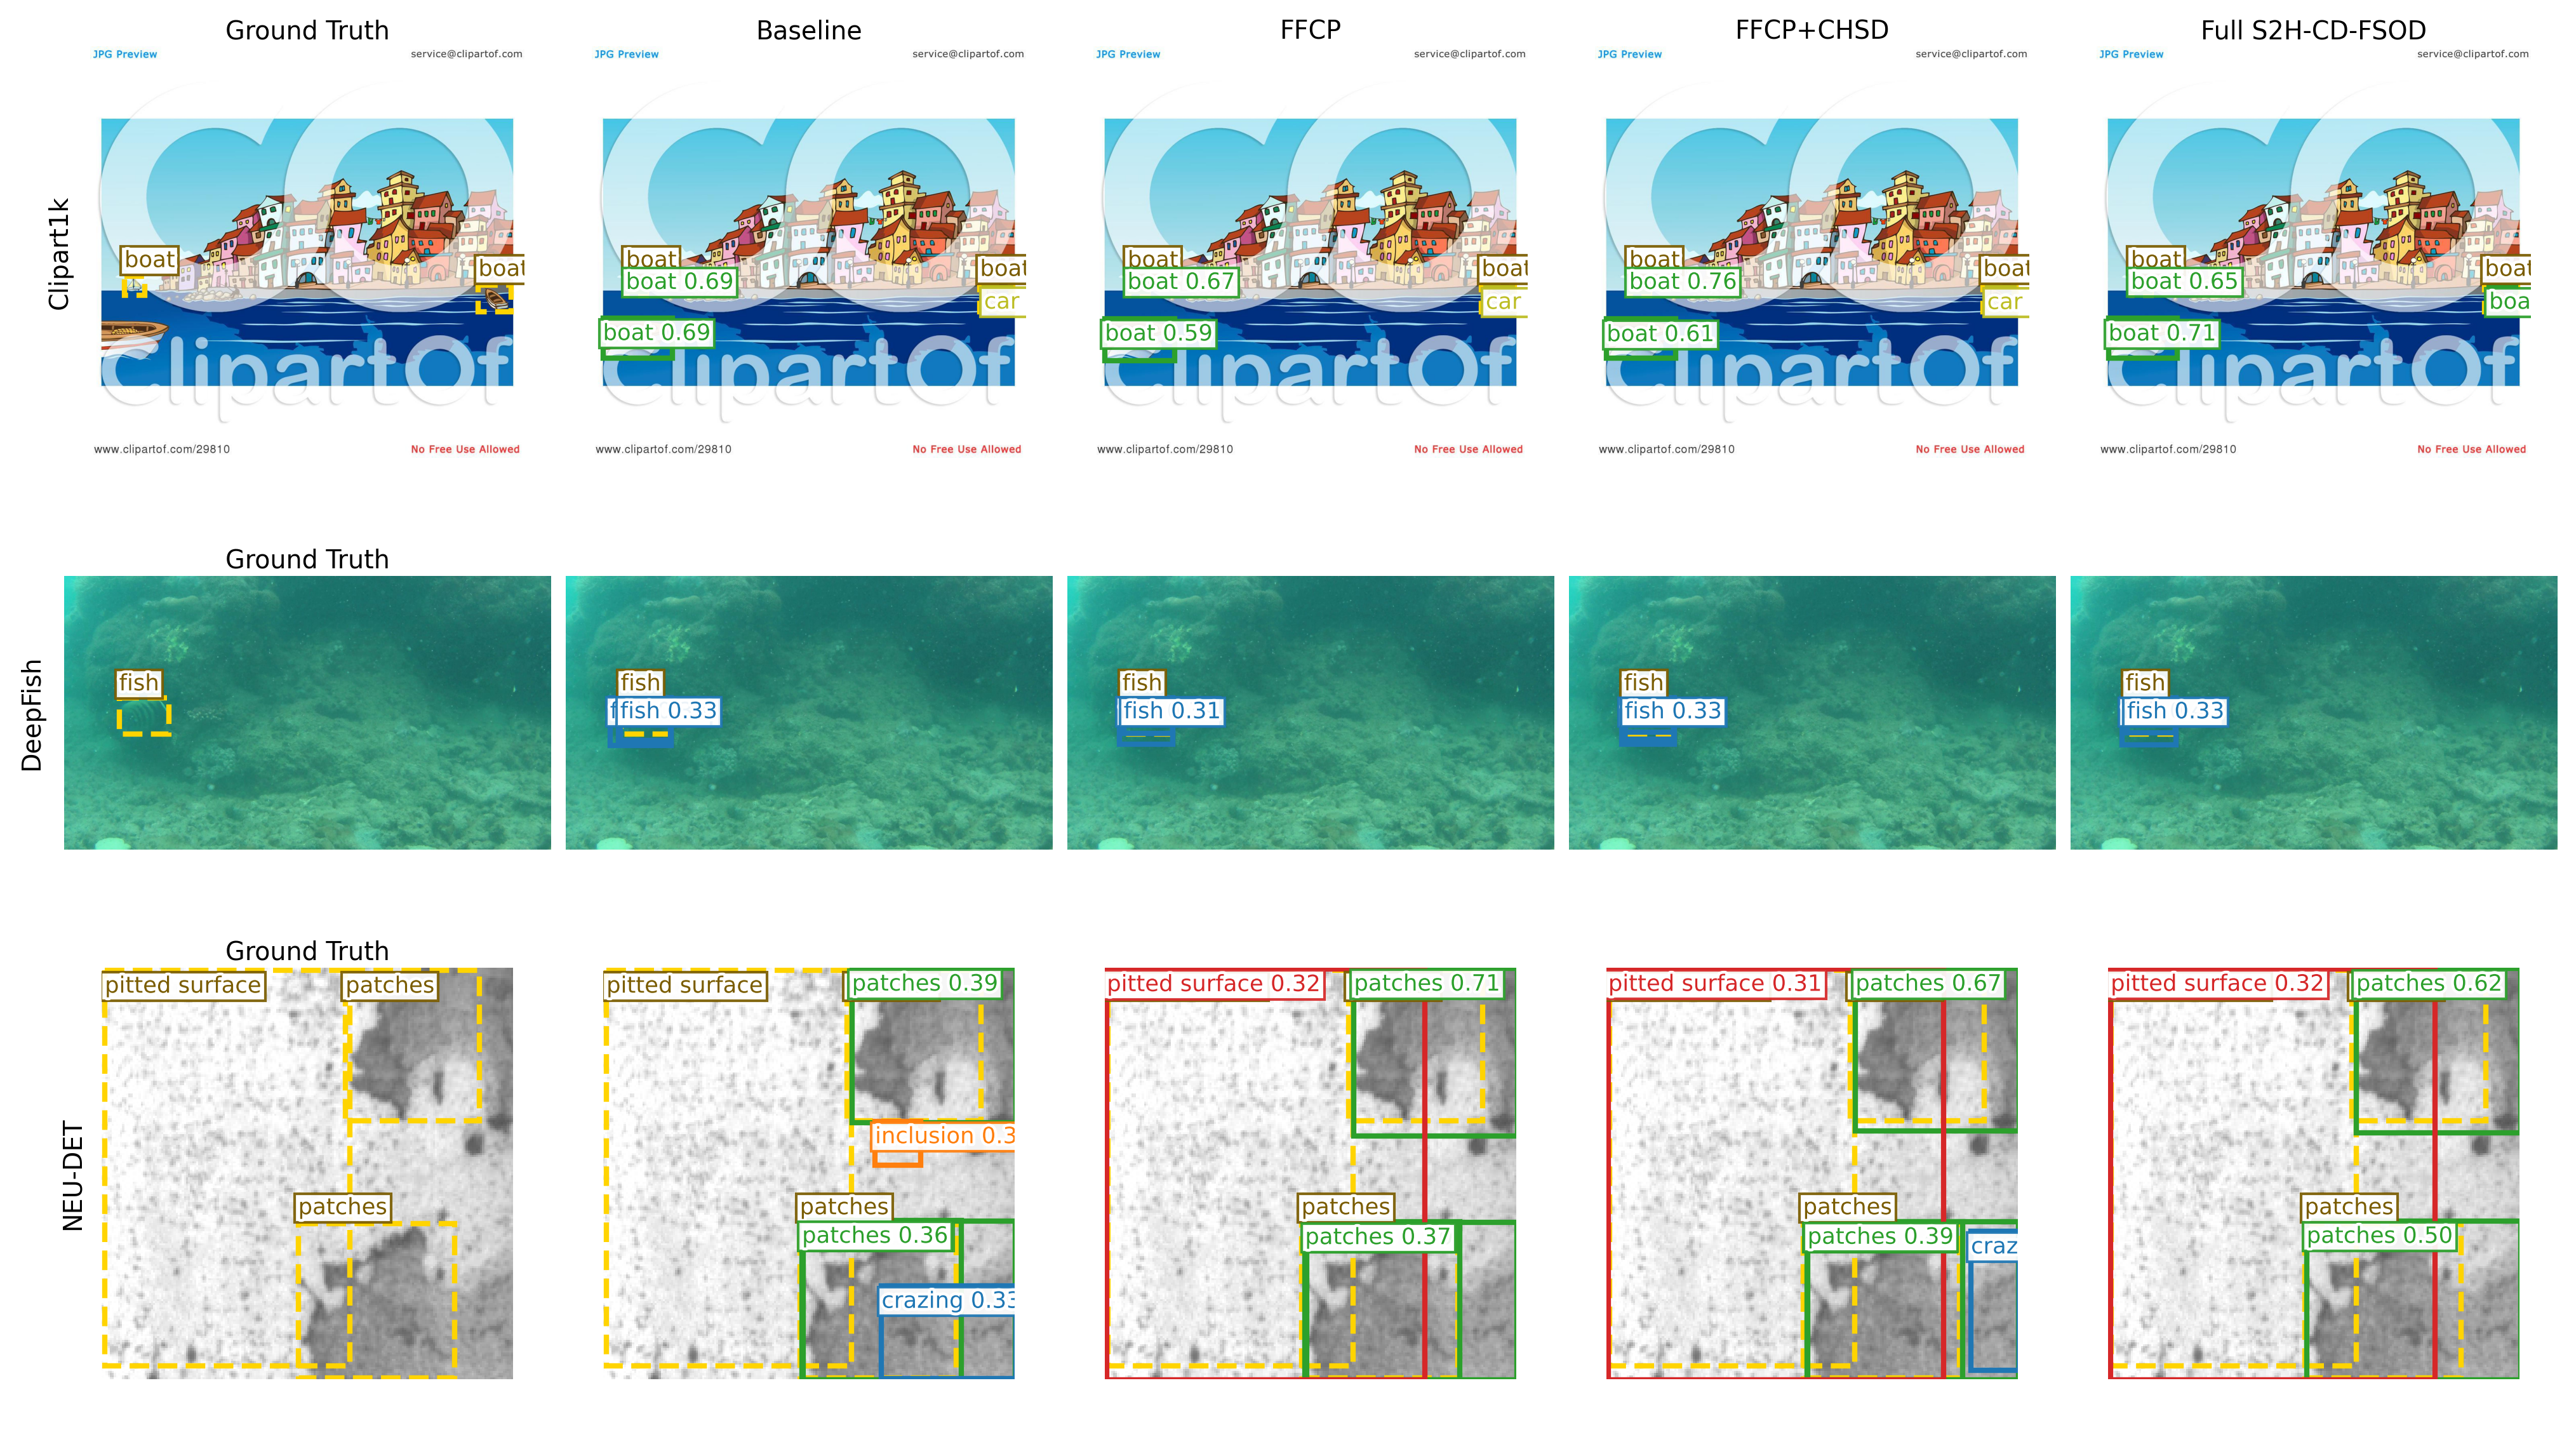
\includegraphics[width=\textwidth]{fig/confidence_progression.png}
    \caption{\textbf{Qualitative detection comparison on 5-shot target domains.}
    Each row shows a representative example from Clipart1k, DeepFish, and
    NEU-DET, while the columns progress from ground truth to the Grounding DINO
    baseline, FFCP, FFCP+CHSD, and the full S2H-CD-FSOD model. Yellow dashed
    boxes indicate annotated objects; colored prediction boxes are labeled with
    the predicted category and confidence score. The examples illustrate how the
    cumulative stages suppress context-driven or spurious responses while
    retaining detections of the target objects, with the largest changes
    occurring in the cluttered underwater and industrial scenes.}
    \label{fig:confidence_progression}
\end{figure*}


We evaluate four cumulative variants under the 5-shot protocol: the fine-tuned
Grounding DINO baseline, FFCP, FFCP+CHSD, and the complete S2H-CD-FSOD model.
All variants share the support splits, optimization budget, and evaluation
code. Fig.~\ref{fig:ablation_map} summarizes the mean mAP of each variant as a
compact cumulative bar group, and Fig.~\ref{fig:confidence_progression}
visualizes the effect of each stage on representative queries. The cumulative
ordering follows the pipeline: FFCP estimates context-sensitive directions,
CHSD builds the identity/appearance decomposition, and ATAR decides how much
authority the retained evidence receives on each query.

Fig.~\ref{fig:ablation_map} reports the quantitative gains for the four
domains with completed ablation runs (Clipart1k, DeepFish, NEU-DET, and UODD);
the baseline bars use the corresponding Grounding DINO$^\dagger$ values from
Table~\ref{tab:main_comparison}, and the remaining bars are the seed-averaged
mAP values of the current run workbook.
AP50 and AP75 are kept in the numerical tables rather than duplicated as plots,
and only completed runs appear.
Fig.~\ref{fig:confidence_progression} presents
qualitative 5-shot comparisons on Clipart1k, DeepFish, and NEU-DET. The
examples show three complementary effects of the cumulative stages:
context-driven duplicate or category responses are reduced, low-contrast target
detections are retained, and industrial defect boxes remain aligned with the
annotated regions. These examples illustrate the kinds of changes measured by
the aggregate results rather than replacing the numerical comparison.

\subsection{Qualitative Analysis}
\label{sec:qualitative}

Following LMP~\cite{lmp}, the main paper keeps a single cross-domain
visualization (Fig.~\ref{fig:confidence_progression}) and defers the remaining
imagery to the supplementary material. The figure uses the same support split,
checkpoint, preprocessing, score threshold, and post-processing for every
column. Clipart1k exposes contextual boat/car confusions, DeepFish stresses a
small low-contrast fish, and NEU-DET contains overlapping defect categories
such as patches, crazing, and inclusions. The intended outcome is a selective
change in error type---fewer context-driven responses and better-supported
category decisions---rather than a blanket increase in the number of
predictions. Cross-domain qualitative comparisons and balanced failure cases
are reported in the supplementary material.
